% Chapter 1
%\label{Chapter1} % For referencing the chapter elsewhere, use \ref{Chapter1} 

%----------------------------------------------------------------------------------------

% Define some commands to keep the formatting separated from the content 
\newcommand{\keyword}[1]{\textbf{#1}}
\newcommand{\tabhead}[1]{\textbf{#1}}
\newcommand{\code}[1]{\texttt{#1}}
\newcommand{\file}[1]{\texttt{\bfseries#1}}
\newcommand{\option}[1]{\texttt{\itshape#1}}
\newcommand{\grados}{$^{\circ}$}

%----------------------------------------------------------------------------------------

\chapter{Introducción general} % Main chapter title
\label{IntroGeneral}

%----------------------------------------------------------------------------------------
% Resumen de capitulo
%----------------------------------------------------------------------------------------

En este capítulo se exponen las problemáticas encontradas con el hardware en el estudio de los Sistemas Embebidos, que motiva la realización de un emulador para la placa EDU-CIAA-NXP \citep{EDU-CIAA-NXP}. Presentando los objetivos, el alcance, los requerimientos y la metodología de trabajo utilizada para llevar a cabo este proyecto.

%----------------------------------------------------------------------------------------
\section{Motivación}
%----------------------------------------------------------------------------------------

Los emuladores son desarrollos de software que modelan el funcionamiento del hardware real, de manera que permiten ejecutar programas dentro de un ambiente que imita su comportamiento \citep{sanchezqemu}. De esta forma un usuario puede simular su código antes de instalarlo en el dispositivo físico.

Para colaborar con la enseñanza de la programación de Sistemas Embebidos, se propuso, como parte del Proyecto CIAA \citep{CIAA}, realizar una plataforma de software que emule el funcionamiento de la placa EDU-CIAA-NXP, así como los periféricos y placas que se pueden conectar a ella.

Esto se debe a que para el desarrollo de aplicaciones en sistemas embebidos es necesario tener de antemano la placa de desarrollo y los componentes de hardware externos a conectar a la placa, para poder probar los programas realizados. Además, muchas veces un usuario sin experiencia, no cuenta con los dispositivos para comenzar, se equivoca en la selección de los mismos, o en las conexiones eléctricas, provocando daños irreparables en el hardware. 

De esta manera, mediante el uso de un emulador se evita todos estos inconvenientes y permite al usuario probar sus programas rápidamente, enfocándose en el desarrollo de aplicaciones y ejecutando sus pruebas en un sistema virtual, dejando para más adelante la implementación en el hardware real.

Un aspecto importante a destacar es el alto costo del hardware y la variedad de dispositivos necesarios. Entonces, contar con un emulador habilita a personas con bajos recursos aprender a programar Sistemas Embebidos utilizando hardware virtual, que se comporta como el hardware real, permitiendo probar diferentes tecnologías.

Para disponibilizar esta herramienta lo más posible, se decidió construir una plataforma de desarrollo con interfaz gráfica dentro de un entorno web, accesible a través de un navegador. De esta manera, se obtiene una herramienta que esté disponible de forma \textit{on line}, para que pueda usarse de forma gratuita, tanto en Computadoras, Tablets o Smartphones, como puede observarse en al figura \ref{fig:EsquemaEmulador}.

\begin{figure}[ht]
	\centering
	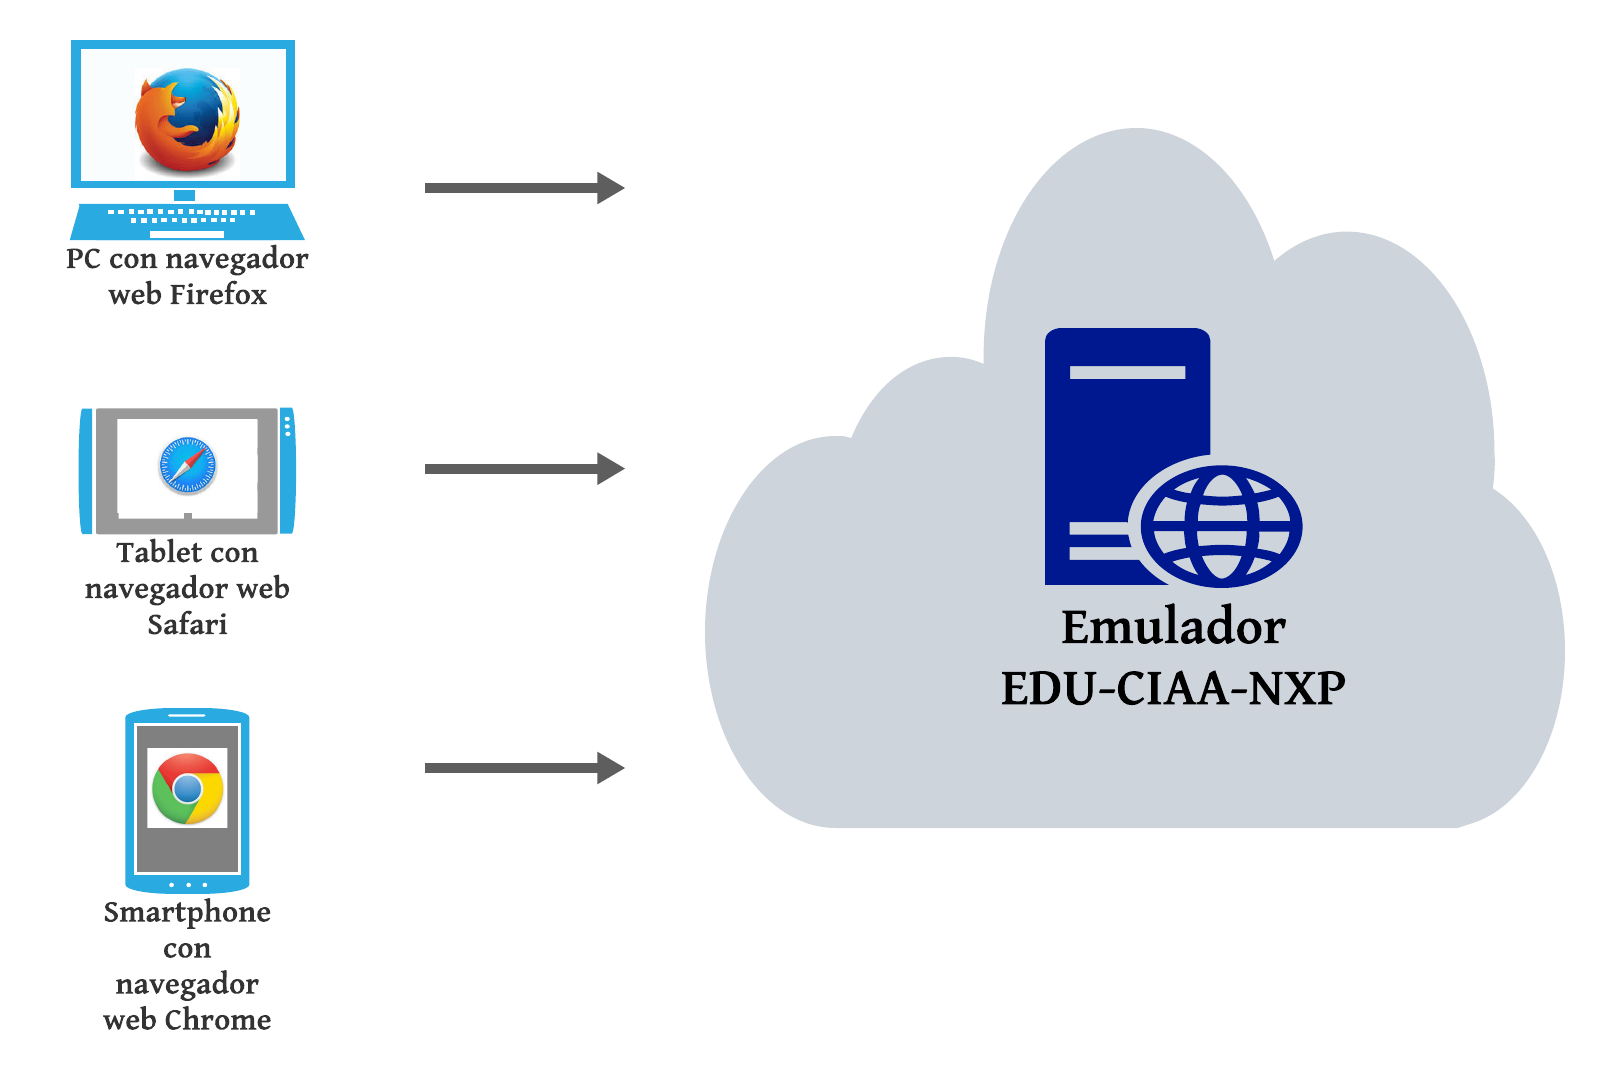
\includegraphics[scale=.55]{./Figures/EsquemaEmuladorCh1.png}
	\caption{Esquema Emulador EDU-CIAA-NXP.}
	\label{fig:EsquemaEmulador}
\end{figure}

En otras palabras, con esta herramienta de emulación, una persona que recién comienza tendrá la experiencia de relacionarse con un sistema embebido solamente conectandose mediante internet a la aplicación web en su ordenador, liberando así el camino a los estudiantes novatos de hacer la interacción con el hardware.

La autora del presente trabajo ha colaborado previamente en el Proyecto CIAA, mediante el desarrollo del software CIAA-BOT Debug como Trabajo Final de la Carrera en Especialización en Sistemas Embebidos de la FI-UBA \citep{TrabajoFinalCESE}, que permite depurar programas realizados mediante el lengaje gráfico CIAA-BOT.

%----------------------------------------------------------------------------------------
\section{Objetivos}
%----------------------------------------------------------------------------------------

Dados los antecedentes explicados, el objetivo de este trabajo es desarrollar una herramienta educativa que brinda un entorno virtual para la placa EDU-CIAA-NXP, permitiendo al usuario seleccionar y conectar con la EDU-CIAA-NXP diferentes tipos de dispositivos virtuales e interactuar con los mismos. Este desarrollo permite al usuario cargar, ejecutar, editar y corregir sus programas escritos en lenguaje C, pudiendo monitorizar gráficamente en la pantalla del ordenador la placa EDU-CIAA-NXP y muchos de los dispositivos de entrada y salida más comunes, todo de manera virtual, sin necesidad de disponer de ningún dispositivo de hardware.

%----------------------------------------------------------------------------------------
\section{Alcance}
%----------------------------------------------------------------------------------------

En el presente trabajo se realizó una primera versión de la herramienta para ser usada con la placa EDU-CIAA-NXP. En particular, se incluyen los siguientes aspectos:

\begin{enumerate}
	\item Desarrollo de aplicación para emular el hardware en PC.
	\item Realización de programas de ejemplo para ser usados dentro de la aplicación.
	\item Documentación de referencia.
\end{enumerate}

El presente proyecto no incluye el desarrollo de la aplicación para emular otras placas que no sea EDU-CIAA-NXP.

%----------------------------------------------------------------------------------------
\section{Requerimientos}
\label{sec:Requerimientos}
%----------------------------------------------------------------------------------------

Se han identificado los siguientes requerimientos:

\begin{enumerate}
    \item Investigación y definición de la arquitectura del software.
        \begin{enumerate}
            \item Investigar sobre las plataformas de emulación de hardware existentes.
            \item Investigar la arquitectura y funcionamiento de las bibliotecas y ejemplos para la EDU-CIAA-NXP, disponibles en firmware v3 \citep{firmwareV3}.
        \end{enumerate}
    \item Desarrollo del Emulador.
        \begin{enumerate}
            \item Realizar la aplicación para emular el hardware.
            \item Integrar las bibliotecas de lenguaje C de la placa EDU-CIAA-NXP portándolas a la paltaforma virtual.
            \item Respetar el estilo de código de las bibliotecas.
            \item Portar ejemplos de utilización de las bibliotecas.
            \item Desarrollar nuevos ejemplos.
        \end{enumerate}
    \item Documentación del proyecto.
        \begin{enumerate}
            \item Elaborar la documentación de la plataforma.
            \item Confeccionar un manual de usuario.
        \end{enumerate}
\end{enumerate}

%----------------------------------------------------------------------------------------
\section{Metodología de trabajo}
%----------------------------------------------------------------------------------------

Para el desarrollo de este trabajo se eligió utilizar las siguientes prácticas:

\begin{itemize}
    \item Utilizar software libre para el desarrollo del proyecto. Reutilizar todo el software y ejemplos disponibles, tanto del Proyecto CIAA como de terceros.
    \item Utilizar un Sistema de Control de Versiones de código fuente distribuído \citep{ControlVersionesGIT}.
    \item Desarrollar \textit{tests} unitarios y de integración.
    \item Automatizar los \textit{tests} y \textit{deployments} mediante Integración Continua \citep{IntegraciónContinuaGIT}.
\end{itemize}
